\documentclass[12pt]{article}
\usepackage[a4paper,margin=1in]{geometry}
\usepackage{graphicx}
\usepackage{amsmath, amssymb}
\usepackage{algorithm, algpseudocode}
\usepackage{multicol}

\usepackage[
backend=biber,
style=numeric
]{biblatex}% For bibliography
\addbibresource{references.bib}

\usepackage{hyperref}
\hypersetup{
    colorlinks=true,
    linkcolor=blue,
    filecolor=magenta,      
    urlcolor=cyan,
    pdftitle={Overleaf Example},
    pdfpagemode=FullScreen,
    }


\newcommand\Tau{\mathcal{T}}
\DeclareMathOperator*{\argmax}{arg\,max}


\title{\textbf{Proposal: Efficient Large-Scale Text Classification with ANN and Transformer Embeddings}}
\author{Collin Zoeller \\ Carnegie Mellon University \\ czoeller@andrew.cmu.edu}
\date{\today}

\begin{document}

\maketitle

\begin{abstract}
Matching text across documents of different sources engenders a unique set of challenges that make confident string matching difficult. Big data analysis introduces other challenges, primarily in memory and computational complexity. Rule-based string distance measures fail to address many idiosyncrasies characteristic of human-written language, resulting in low-confidence matches. Sentence transformers capture these nuances effectively, but state-of-the-art methods become computationally expensive at scale due to the $O(nm)$ complexity of pairwise matching. Since our project requires the classification of over 1 billion strings from administrative data, standard classification approaches such as cosine similarity are infeasibly expensive. 
This paper proposes leveraging an open-source transformer model with approximate nearest neighbor (ANN) for efficient classification. Using ANN’s $O(\log(n))$ complexity, this approach balances accuracy and computational efficiency, enabling scalable and effective text matching for large-scale data.
\footnote{This is an adaptation of a proposal for a project utilizing IRS data. Specific references to the details of IRS internal processes and data are omitted, and the process is generalized for large-scale text classification of administrative data.}  
\end{abstract}
\clearpage
\section{Introduction}\label{sec:intro}

The objective of this project is to create a highly accurate string match between a list of user-inputted occupation titles and a list of target occupation classes.  As a classification problem, this is a complex challenge, particularly given the vast scale of the data. With an input size of more than 1 billion observations and 969 possible target categories, traditional approaches do not efficiently meet this objective. 

This project aims to develop a highly accurate classification model that maps user-submitted occupations to their correct classifications. Specifically, we seek to learn a function:
\begin{align*}
   &f(x): x \mapsto y \in Y, \quad \forall x \in X\\
    &X:  \text{Space of Input Strings}\\
    &Y: \text{Set of Target Classifications}
\end{align*}

Four major considerations guide our approach:

\begin{enumerate}

    \item \textbf{Natural Language}. Human language is characterized by noise such as misspellings, abbreviations, synonyms, unconventional formatting, and superfluous text. Rule-based approaches, recurrent neural networks and early transformers are unable to handle these nuances. We explore the state-of-the-art transformer-based embeddings from small language models as the most accurate representation of the semantic meaning of the input strings.
    \item \textbf{Scale}. Given that $|X|$ ranges between 500 million and 1.3 billion, the solution must be computationally efficient, scalable, and replicable. We explore approximate nearest neighbors as an effective approach for efficient clustering in large feature spaces. 
    \item \textbf{Evaluation Metrics}. Misclassification can have downstream impacts including bias in subsequent econometric analyses. Model performance must be evaluated using precision, recall, F1-score, and accuracy to ensure reliable predictions.
    
\end{enumerate}

In this paper, we propose a scalable approach that leverages sentence embeddings and approximate nearest neighbors to efficiently map user-inputted occupation titles to one of 969 categories.

The rest of this paper is organized as follows. The remainder of Section \ref{sec:intro} discusses the background and motivation of the transformer model, approximate nearest neighbors, and the evaluation metrics. Section \ref{sec:methodology} describes the methodology of the proposed solution, including embeddings and model training and evaluation. Section \ref{sec:outcomes} discusses the expected outcomes of developing the proposed solution, both in the scope of the project and beyond it. Section \ref{sec:timeline} provides a conservative timeline for completion of the project.



\subsection{Pitfalls of Classical Rule-based Approaches}

Rule-based string similarity measures have long been a cornerstone of natural language processing. These methods rely on well-defined mathematical formulations. 
However, they fail in complex classification tasks due to their reliance on surface-level text properties rather than true semantic meaning.

For example, Jaro-Winkler Similarity calculates a score based on the number of matching characters and transpositions between two strings, assigning higher similarity to shorter edits and giving preference to common prefixes. The similarity between strings $s_1$ and $s_2$ is mathematically given by Equation \ref{eq:jaro} where  $|M|$  is the number of matching characters and  $T$  is the number of transpositions.

\begin{align} \label{eq:jaro}
    J(s_1, s_2) = \frac{1}{3} \left(\frac{|M|}{|s_1|} + \frac{|M|}{|s_2|} + \frac{|M - T|}{|M|} \right)
\end{align}


In contrast with similarity measures, Edit-distance approaches, such as the Levenshtein distance, quantify similarity by counting the minimum number of operations (insertions, deletions, and substitutions) required to transform one string into another.
Edit distances perform poorly between similar proper nouns, such as business names and titles, because transposed, inserted, or omitted words exacerbate the distance. For example: 

\begin{center}
    Global Insurance Co. \\vs.\\ 
    Global (Asset) Insurance. 
\end{center}
Here, the addition of ``(Asset)" and the removal of ``Co." added 7 characters and removed 3, resulting in 10 operations. This is problematic for an editing distance. There are adaptions, like bag-of-words, that perform the same measures at a token (word) level, but then encounter issues of misspellings and other errors at the character level. 

One of the most effective classical measures is cosine similarity, which treats strings as vectorized representations in a high-dimensional space, often using the term frequency-inverse document frequency (TF-IDF) or character-level n-grams (groups of n-characters, including white space). The similarity score is a correlation computed as the cosine of the angle between two vectors A and B :

\begin{align}
    \cos(\theta) = \frac{A \cdot B}{\|A\| \|B\|}
\end{align}
Dissimilar strings have a score of -1, identical strings have a score of 1. 

Still, cosine similarity does not consider word order. In the example below, both occupations would have a high cosine similarity despite their different meanings.

\begin{center}
    Architect Consultant\\vs.\\
    Consultant Architect
\end{center}


Cosine similarity is often considered the baseline for many NLP tasks because of its simplicity: It is easier to say that two strings are 80\% similar than that two strings are 5 edits away from each other. The issue arises in encoding the strings in such a way that cosine can capture contextual nuances. All rule-based approaches are inherently limited—they depend on surface-level features and fail to capture the deeper relationships between words such as synonyms (including abbreviations), homophones, and contextual meaning.




%%%%%%%%%%% TRANSFORMERS %%%%%%%%%%%%%
\subsection{The Transformer}\label{sec:transformer}
To overcome many of the problems associated with the rigidity of rule-based approaches, most NLP tasks historically used an adaptation of the neural network called the recurrent neural network (RNN) that could encode some positional and contextual information. Introduced in 2017, the Transformer model surpassed the RNN in several ways: 
\begin{enumerate}
    \item the encoding-decoding architecture enables a probabilistic representation of word sequences, rather than considering words or characters in isolation
    \item RNNs typically included Long Short-Term Memory (LSTM) to encode positional information about each word. LSTMs struggle with long-range dependencies due to vanishing gradients and high computational cost.
    \item The self-attention mechanism allows transformers to weigh the importance of words in a sentence based on their relationships to all other words, enabling a richer contextual understanding
    \item Positional encoding enhances attention by providing a measure to the value of words depending on their position in the sequence. For example, 
    \begin{center}
        Lawyer Doctor vs. Doctor Lawyer \end{center}
A \textbf{lawyer doctor} is a legal expert with a doctorate in law (e.g., Juris Doctor, JD) and a \textbf{doctor lawyer} is a medical professional who later became a lawyer or someone who specializes in medical law.
\item Transformers are "pre-trained," meaning that general-use, open-source Transformers can be shared and applied to a wide breadth of use cases. Instead of retraining the model, \textbf{Transformers can be tuned to specialize in domain-specific tasks.} For example, a doctor could tune a model to specialize in (and be most accurate for) understanding potential diseases given a differential diagnosis such as a set of symptoms. 
\end{enumerate}

Figure \ref{fig:attention_arch} illustrates the Transformer architecture\footnote{The process used to develop an output given some textual input.}, which consists of two main components: an encoder and a decoder. A Transformer can contain either or both components. An encoder Transformer (e.g. BERT) creates a vector representation of the text (embedding),  the decoder (e.g. GPT, Llama) creates a probabilistic sequence of strings given an input, and a sequence-to-sequence (or seq2seq) model does both. A simpler representation of the architecture is presented in Figure \ref{fig:encode-decode}.
\begin{figure}
    \centering
    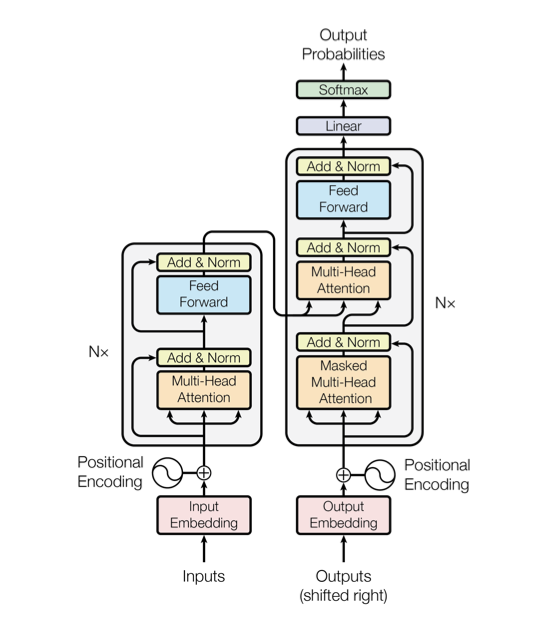
\includegraphics[width=0.5\linewidth]{images/architecture.png}
    \caption{Transformer architecture as proposed by the original authors \cite{DBLP:journals/corr/VaswaniSPUJGKP17}}.
    \label{fig:attention_arch}
\end{figure}

\begin{figure}
    \centering
    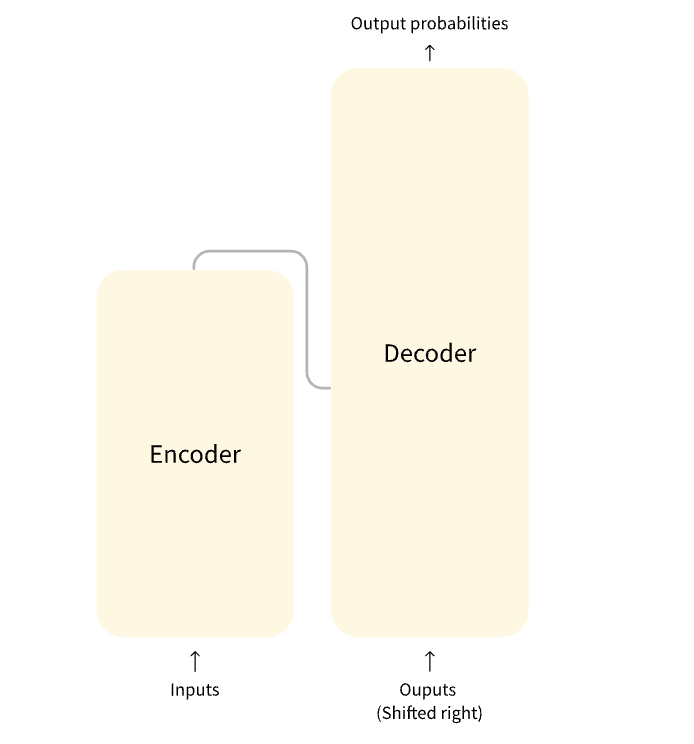
\includegraphics[width=0.5\linewidth]{images/transformers_blocks.png}
    \caption{Encoder-decoder components. Image from Hugging Face\cite{huggingface}.}
    \label{fig:encode-decode}
\end{figure}
The Transformer is the foundation of today's language models and is considered state-of-the-art technology in terms of natural language processing (NLP). Many open-source models are available, but each is usually built with different tasks in mind. Each model also varies in size depending on the number of internal parameters (or weights) required for training. Large language models (LLMs) like GPT (Generative Pre-trained Transformer) use transformer decoders generalized for chatbots and contain hundreds of billions or trillions of parameters, far beyond the capacity of many computers to handle. Small language models (SLMs) are smaller and more versatile models designed for encoder tasks, making them better suited for tasks such as sentiment analysis, semantic similarity, text classification, and summarization, while only containing hundreds of millions of parameters. MiniLM, a general class of SLM, has several models optimized for NLP processes such as semantic similarity and text classification\cite{minilm}. One encoder model, All MiniLM, is known to perform exceptionally well for short-text characteristics while remaining relatively lightweight.


%%%%%%%%%%%%%%%%%%%%%% APPLICATIONS %%%%%%%%%%%%%%%%%%%%%% 
\subsection{Approaches and Applications to Text Classification}\label{sec:techniques}

There are a few ways to apply Transformers to text classification and similarity analysis. 

\begin{enumerate}
    \item A common baseline is to pass the text input and class labels into an encoder model (like BERT or MiniLM), calculate the cosine similarity between the input embeddings and all of the label embeddings, and then select the label with the highest score. This straightforward approach identifies the most semantically similar strings. \label{app1}

    \item Embeddings could be clustered and predicted using the nearest class. Like cosine similarity, this approach also identifies the semantically closest strings. Unlike cosine similarity, this method does not require iterating the labels for every observation, making it a much more efficient alternative. \label{app2}
    
    \item  A specially tuned decoder model may be able to determine semantic similarities from a prompt-based approach. For example:
\begin{quote}
    System role: You are an expert in text classification. Only output the answer. Use this list: $<[list]>$\\
    Prompt: Which item is this string most similar to? $<string>$
\end{quote}
While the model does not explicitly generate embeddings like an encoder-based method, it internally represents the input in a way that allows the model to identify a probabilistically similar string. This is a common approach to NLP used in the SpaCy library \cite{spacy}

\item  It is also feasible to use the embeddings to design a (simple) neural network for text classification. In this network, an additional weight is trained on the input embeddings to yield the correct probability of a class (the softmax). This method requires supervised training but offers a more robust and replicable classifier. \label{app4}

\end{enumerate}

In any of these approaches, the core principle remains the same: leveraging embeddings or probabilistic text outputs to determine the most semantically similar class for a given input.


%%%%%%%%%%%%%%%%%%%%%% SCALE %%%%%%%%%%%%%%%%%%%%%% 
\subsection{Additional Challenges at Scale}\label{sec:ANN}
Once a model is determined and trained/tuned, the process of classifying the text is trivial. Algorithm \ref{alg:class1} demonstrates the classification process for approaches \ref{app1} and \ref{app3}, where $f(x,y)$ is the selected model function. Although this is a valid approach, the complexity of this pairwise matching algorithm is $O(nm)$. In other words, the list of labels is searched in every iteration. This is infeasible for large input spaces such as administrative records.

\begin{algorithm}[hbt!]
\caption{Pairwise Similarity}\label{alg:class1}
\begin{algorithmic}
\Require
\Statex A set of input data \( X = \{ \mathbf{x}_1, \mathbf{x}_2, \dots, \mathbf{x}_n \} \subset \mathbb{R}^d \)
\Statex A set of reference labels \( Y = \{ \mathbf{y}_1, \mathbf{y}_2, \dots, \mathbf{y}_m \} \subset \mathbb{R}^d \)
\Ensure
\Statex Predicted label assignment for each input \( \mathbf{x}_i \)
\For{$i = 1$ to $n$} \Comment{Iterate over each input sample}
    \State $S \gets \emptyset$ \Comment{Initialize an empty similarity score list}
    \For{$j = 1$ to $m$} \Comment{Compare against each reference label}
        \State $ f(\mathbf{x}_i, \mathbf{y}_j) \to \hat{y}_{i,j}$ \Comment{Compute similarity score }
        \State $S            \gets S \cup \{ \hat{y}_{i,j} \} $ \Comment{Append similarity score to list}
    \EndFor
    \State Determine the predicted class: $\hat{y}_i \gets \arg\max S $
\EndFor
\end{algorithmic}
\end{algorithm}

Algorithm \ref{alg:class2} shows the much more direct approaches \ref{app2} and \ref{app4}. These approaches classify $X$ in linear time. Both require an additional step of training prior to classification. 

\begin{algorithm}[hbt!]
\caption{Direct Classification}\label{alg:class2}
\begin{algorithmic}
\Require
\Statex A set of input data \( X = \{ \mathbf{x}_1, \mathbf{x}_2, \dots, \mathbf{x}_n \} \subset \mathbb{R}^d \)
\Statex A trained classifier \( f: \mathbb{R}^d \to Y \) that maps inputs to labels
\Ensure
\Statex Predicted label assignment for each input \( \mathbf{x}_i \)
\For{$i = 1$ to $n$} \Comment{Iterate over each input sample}
    \State $\hat{y}_i \gets f(\mathbf{x}_i)$ \Comment{Compute the predicted label}
\EndFor
\end{algorithmic}
\end{algorithm}

There is a much faster unsupervised technique that is better suited for big data and can perform in sublinear time. The approximate nearest neighbors (ANN) algorithm leverages attributes of both K-nearest neighbors and random forest decision trees. Originally created for Spotify similarity searches, the ANNOY ("Approximate Nearest Neighbors Oh Yeah") algorithm shown in algorithm \ref{alg:annoy} is an ANN that is efficient and intuitive for big data \cite{ANNOYBern}. Although perhaps not obvious, ANNOY performs at $O(\log(n))$, a significant improvement over a more direct classification approach. 

The speedup is primarily a result of how ANN searches the tree. Where in a normal decision tree the optimal class requires an exhaustive search of the entire tree, ANN only considers branch paths that follow the criteria. 

\begin{algorithm}
\caption{ANNOY-Based Classification}\label{alg:annoy}
\begin{algorithmic}[1]

    \Require Dataset $X$ with labels $Y$, number of trees $T$, number of neighbors $k$
    \Ensure Trained ANNOY index for classification
    
    \State Initialize an empty index $I$
    \For{$t = 1$ to $T$} 
        \State Randomly sample a subset $S \subseteq X$
        \State Build a tree recursively:
        \Function{BuildTree}{$S$}
            \If{$|S| \leq \text{min\_leaf\_size}$} 
                \State Return a leaf node storing $(S, Y_S)$, where $Y_S$ contains class labels of $S$
            \EndIf
            \State Choose a random hyperplane by selecting two points at random and computing the normal vector
            \State Partition $S$ into $S_L$ and $S_R$ based on the hyperplane
            \State Create a node storing the hyperplane and left/right child pointers
            \State Assign $\text{left} \gets \textsc{BuildTree}(S_L)$, $\text{right} \gets \textsc{BuildTree}(S_R)$
            \State Return the constructed node
        \EndFunction
        \State Store the root node of the tree in $I$
    \EndFor

    \Function{Classify}{$x, I, k$}
        \State Collect $k$ nearest neighbors from trees in $I$
        \State Obtain their corresponding labels $Y_k$
        \State Predict the majority class in $Y_k$ (or use weighted voting)
        \State Return predicted class
    \EndFunction
    
    \State Return the trained index $I$
\end{algorithmic}
\end{algorithm}

Just as a random forest reduces bias by building a set (a forest) of decision trees trained on random partitions of the training data, an ANN creates a set of randomly partitioned KNN decision trees\footnote{KNN, like other unsupervised models, is a clustering method that is equivalently represented as a decision tree. Although Figure \ref{fig:ANN} shows clusters in 2 dimensions, I refer to KNN and ANN as trees for consistency.} like the one shown in Figure \ref{fig:ANN} on random subsets of the training data. Like KNN, ANN classifies the points based on the majority vote of the $k$-nearest neighbors in each tree and then returns the majority class across trees. Table \ref{tab:ANN-class} lists the decisions for some $\mathbf{x_i} \in \mathbf{X}$ (the input space) with $k=4$ of an example ANN that produced $\Tau = 5$ trees. Because 4 of the 5 trees labeled the observation as belonging to $R1$, the ANN will classify this observation as $R1$.

\begin{table}
    \centering
    \begin{tabular}{|c|c|c|c|c|c|}
      \hline
      Tree & 1 & 2 & 3 & 4 & Decision\\
      \hline
       1  & R1 & R1  & R1 & R3 & R1\\
       2  & R2 & R1  & R3 & R1 & R1\\
       3  & R1 & R2  & R2 & R2 & R2\\
       4  & R3 & R4  & R2 & R1 & R1\\
       5  & R3 & R1  & R2 & R1 & R1\\
       \hline
    \end{tabular}
    \caption{Example ANN Classifying Criterion}
    \label{tab:ANN-class}
\end{table}

\begin{center}
    

\end{center}
\begin{figure}
    \centering
    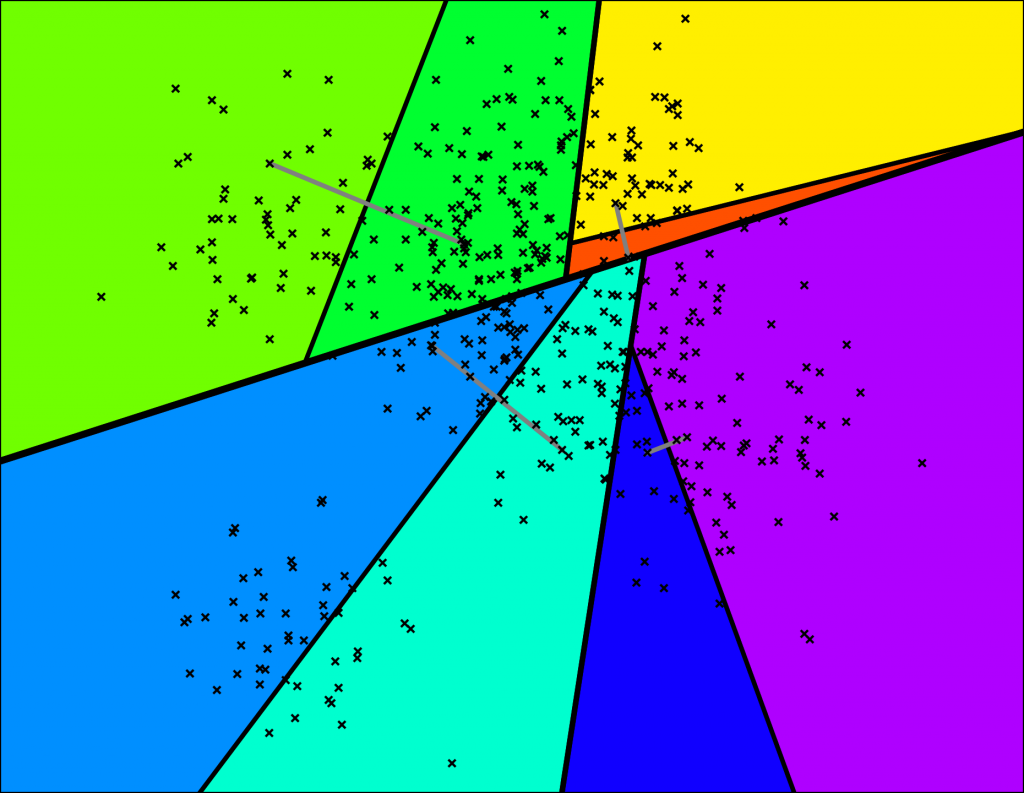
\includegraphics[width=0.5\linewidth]{images/tree-3-1024x793.png}
    \caption{Single Iteration of ANN Clustering \cite{ANNOYBern}}
    \label{fig:ANN}
\end{figure}


\subsection{Model Evaluation}
The number of assessments for the performance of the language model is as varied as the tasks assigned to them. There is an additional layer of complexity given the vastness of data used to train models, as model evaluations of any machine learning approach should measure model effectiveness on out-of-sample observations (those not used to train or tune the model). 

For text classification tasks, LLMs can be evaluated with the same criteria as other classical approaches: accuracy, precision, recall, and F1 scoring. 

\begin{align*}
    &\textbf{Accuracy:  } \frac{\text{TP}}{\text{TP + TN + FP + FN}} \\
    & \textbf{Precision:  } \frac{\text{TP}}{\text{TP + FP}}\\
    &\textbf{Recall:  }\frac{\text{TP}}{\text{TP + FN}}\\
    &  \textbf{F1:  }  \frac{2 \times \text{Precision}\times \text{Recall}}{\text{Precision + Recall}}
\end{align*}

In all cases, the score is in the range $[0,1]$ where a score close to 1 is preferred. Heuristically, a classifier with an F1 score greater than $0.8$ is considered a good model. Transformer models have been proven to increase this to $0.9$ or more\footnote{Most studies using Transformers on text classification use the BERT Transformer model or one of its offshoots, which are among the more "primitive" architectures. More recent models may yield even higher scores.} \cite{lu2022comparative}\cite{transformer-text-class}\cite{gokhan-trans-text-class}. 

\section{Methodology}\label{sec:methodology}
This project assists in collecting the data necessary for a subsequent economic analysis of the heterogeneous effects of previous occupations on firm founding. The objective of this project is to create a mapping of varied and noisy self-reported occupation titles to a structured set of ONET\footnote{\href{https://www.onetonline.org/find/all}{https://www.onetonline.org/find/all}} occupation classifications. We frame this task as a high-dimensional text classification problem and propose a scalable machine learning approach.

\subsection{Problem Definition}

Let $X$ be the set of all reported occupation titles, and let $Y$ be the set of 969 ONET occupation categories derived from Dingel and Neiman's\footnote{See \href{https://github.com/jdingel/DingelNeiman-workathome/occ_onet_scores/output/occupations_workathome.csv}{https://github.com/jdingel/DingelNeiman-workathome/occ\_onet\_scores/}} dataset \cite{DINGEL2020} . 
Our goal is to construct a mapping function:
\[
f: X \to Y
\]
such that each occupation title in $X$ is assigned to the most semantically similar category in $Y$. Given the vastness of the text data (over a billion observations), a rule-based approach is infeasible, and pairwise similarity approaches and supervised learning methods are inefficient. Instead, we leverage transformer-based text embeddings from a specialized small language model (SLM) and an Approximate Nearest Neighbor (ANN) search for efficient classification.


\subsection{Proposed Pipeline}
We propose the following methodology:

\begin{enumerate}
    \item Encode occupation titles and ONET categories into dense vector embeddings using the \texttt{All-MiniLM} Transformer.
    \item Build the ANN index using ANNOY algorithm on the ONET class categories
    \item For each feature embedding, search the ANN for the nearest class embedding.
    \item Perform hyperparameter tuning and model selection based on F1-score, iterating until a performance threshold of 98\% is met or there is no significant improvement.
\end{enumerate}

The returned results from the final model is considered the mapping from the user-inputted list of occupation titles to those listed in ONET. 

All code is written in Python and housed internally for confidentiality. A demonstrative version using synthetic and publicly available scraped data is hosted on Github \footnote{See the repository at \href{https://github.com/ColZoel/Annoy_text_classifier}{https://github.com/ColZoel/Annoy\_text\_classifier}}. 

\subsubsection{Special Considerations: Unseen Categories}
Given the vastness of the input space, many self-inputted occupations do not fit any of the categories provided in the output space. For example, "Student" and unpaid domestic work such as "Homemaker" or "Housewife" appear frequently in the data. Introducing these and other commonly omitted occupations as additional labels is feasible before embedding the output space. 

Additionally, noise such as unnecessary numbers, punctuation, special characters, and non-English script can reduce the effectiveness of any model. While the administrative data considered here does not face this issue, it is generally good practice to process the text before encoding the embeddings. 


\begin{figure}
    \centering
    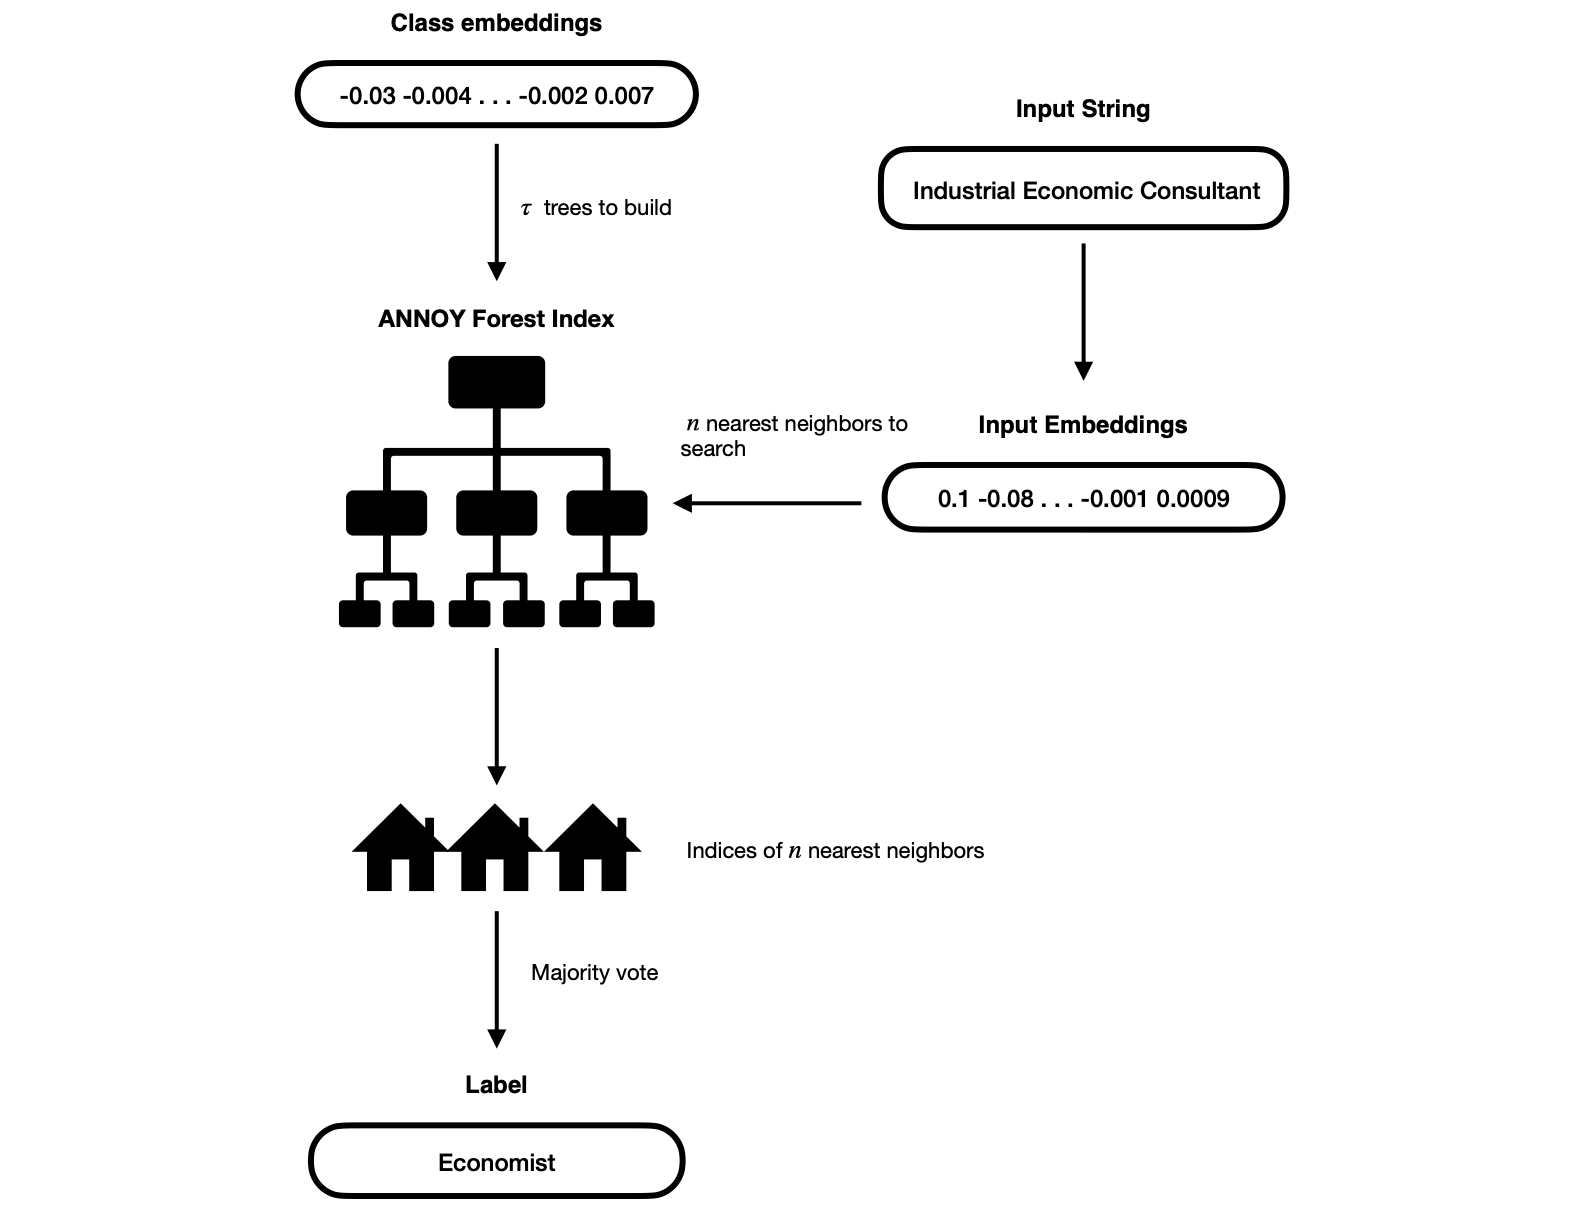
\includegraphics[width=0.9\linewidth]{images/pipe_black.jpeg}
    \caption{Simple Method Pipeline}
    \label{fig:pipe}
\end{figure}


Now we address each item in turn.

\subsection{Encode with All MiniLM}

\textbf{Packages needed:} \begin{verbatim}
sentence-transformers
\end{verbatim}
alternatively, 
\begin{verbatim}
    transformers
    torch
\end{verbatim}

\textbf{Models to consider}\footnote{These models seem to perform best for short text. Their differences are nuanced, but all are capable of text classification. A comparison of model performance and sizes is available at \href{https://www.sbert.net/docs/sentence_transformer/pretrained_models.html}{https://www.sbert.net/docs/sentence\_transformer/pretrained\_models.html}}:
\begin{verbatim}
    all-MiniLM-L6-v2
    all-MiniLM-L12-v2
    all-mpnet-base-v2
\end{verbatim}

The first step involves encoding the input and target occupation classes using the All-MiniLM Transformer model. All-MiniLM is a lightweight and efficient sentence-transformer model optimized to generate dense embeddings, making it suitable for large-scale text classification tasks. Since the Transformer is pre-trained (see Section \ref{sec:transformer}), the semantic information for every observation in both $X$ and $Y$ is "baked into" the model, meaning no additional training is required to return an appropriate numeric representation of the text.

\subsubsection{Why MiniLM?}
\begin{itemize}
    \item \textbf{Efficiency:} MiniLM is designed to retain the effectiveness of larger Transformer models while significantly reducing computational overhead. Effective model sizes are between 80 and 200MB and can encode between 7,500 and 14,000 sentences per second. 
    \item \textbf{Semantic Representation:} The model produces dense embeddings that capture the semantic similarities between text inputs. These are 384-dimensional vectors that encode the position and other characteristics of each word.
    \item \textbf{Versatility:} Pre-trained on a broad range of text data (over 1 billion observations), making it applicable to occupation classification tasks and unlikely to need tuning. 
\end{itemize}

\subsubsection{Encoding Process}
Given an occupation title \(x_i\) and ONET occupation labels \(y_j\), the encoding process follows:

\begin{enumerate}
    \item Load the pre-trained All MiniLM model.
    \item Convert each occupation title and ONET label into vector representations using the model.
    \item Store the resulting vectors for ANN prediction
\end{enumerate}

Each $x \in X$ and $y \in Y$ is now represented in a high-dimensional space, allowing efficient similarity comparisons.

\subsection{Training an Approximate Nearest Neighbor Model}

\textbf{Packages:}
\begin{verbatim}
    annoy
\end{verbatim}

An ANN model is trained using the ANNOY algorithm. The steps involved include:

\begin{enumerate}
    \item Construct multiple random projection trees from occupation embeddings.
    \item Index all target labels using the same tree structure.
    \item Query the ANN model to return the top \(k\) nearest ONET matches for each occupation title.
\end{enumerate}

The ANN approach allows for efficient large-scale classification with sublinear search time (see Section \ref{sec:ANN}). Unlike clustering approaches, the tree is only built on the ground truth (outcome) and not the entire embedding space. Each point is classified according to its proximity to a given output embedding, which can reduce the bias associated with cluster size.

Hyperparameter selection follows a randomized search technique \cite{bergstra12a_randomSearch}. This technique is known to quickly converge to an optimal combination (although not necessarily a globally optimal combination). 

\subsection{Model Comparison and Selection}

Model are evaluated by measurement of F1 scores in different hyperparameter configurations on random samples of the produced tree. The configuration with the highest F1 score is selected. While the goal is a score of 0.98, there is a trade-off with hyperparameter exploration and time. An acceptable interval of [0.9-0.99] would allow the model with the best score to be selected after a maximum of $n$ iterations. In other words, we use the following selection rule:

\begin{algorithm}
\caption{Model Selection}\label{alg:annoy}
\begin{algorithmic}[1]
    \For{$i=1$ to $n$}
    \State Train ANN on new (randomized) hyperparameter configuration $\to f_i(x)$
    \State Select random $\mathbf{x} \subset \mathbf{X}$
    \State $f_i(\mathbf{x}) \to \mathbf{\hat{y}}_i$
    \Comment{query subset results}
    \State GETSCORE($\hat{\mathbf{y}}_i, \mathbf{y}_i $) $\to S_i$
    \If{$S_i >= 0.98$}
    \State Return $f_i(x)$
    \EndIf
    \If{$i==n$}
    \State Return $\argmax(S)$\
    \EndIf
    \EndFor
\end{algorithmic}
\end{algorithm}

The selected model is considered the best-in-class. At this point, we can query each point and return the indicated label, return these to a structured form such as CSV, Parquet, or a Stata dataset, and associate them with the panel data. 


\section{Expected Outcomes}\label{sec:outcomes}

The proposed methodology aims to develop a scalable and efficient classification model for mapping occupation titles to ONET categories. The expected outcomes of this approach are as follows:

\begin{enumerate}
    \item \textbf{High-Performance Occupation Classification:} 
    The final model is expected to achieve an F1 score of at least 98\%, ensuring accurate occupation classification.

    \item \textbf{Scalability for Large Datasets:} 
    By leveraging the efficiency of Transformer-based embeddings and approximate nearest neighbor search, the selected model should be capable of handling large occupation datasets with minimal computational overhead.

    \item \textbf{Benchmark Comparison of Classification Methods:} 
    This approach will provide a case analysis of short text classification at scale using MiniLM embeddings, which is not well studied in the literature. Both techniques have been applied and studied separately on long text (sentences or greater) but never together.  

    \item \textbf{Optimized Hyperparameter Configurations:} 
    The research will yield insights into optimal hyperparameter settings for both models, including the number of ANN trees and the number of neighbors (\(k\)).

    \item \textbf{Potential for Generalization to Other Text Classification Tasks:} 
    While the study focuses on occupation classification, the techniques developed may be applicable to other large-scale text classification applications.

\end{enumerate}

In general, the research aims to contribute a robust and scalable methodology for occupation classification, offering valuable insights into text classification techniques using modern Transformer-based embeddings and approximate nearest-neighbor search.

\section{Timeline}\label{sec:timeline}
These are conservative maximum time estimates. Most items would take less than the indicated time, but this allows room for unknown difficulties.
\begin{table}[h]
    \centering
    \begin{tabular}{|c|c|}
        \hline
        Phase & Duration \\
        \hline
        Data Pull from CDW & 2 Days \\
        Request missing packages & 1 Day \\
        Build Pipeline & 1 Week \\
        Train and Evaluate ANN & depends on $n$; 1 Week \\
        Return Final Mapping & 1 Day\\
        \hline
    \end{tabular}
    \caption{Proposed Timeline}
    \label{tab:timeline}
\end{table}

If for some reason this approach fails, a backup solution using embeddings and neural networks will be used. In that event, a new proposal or white paper will be provided.  

\newpage
\nocite{*}
\printbibliography

\end{document}
